%\section{Runtime Architecture}

\section {The NFVactor Framework}
\label{sec:nfvactor-runtime-and-controller}

\begin{figure}[!t]
  \centering
  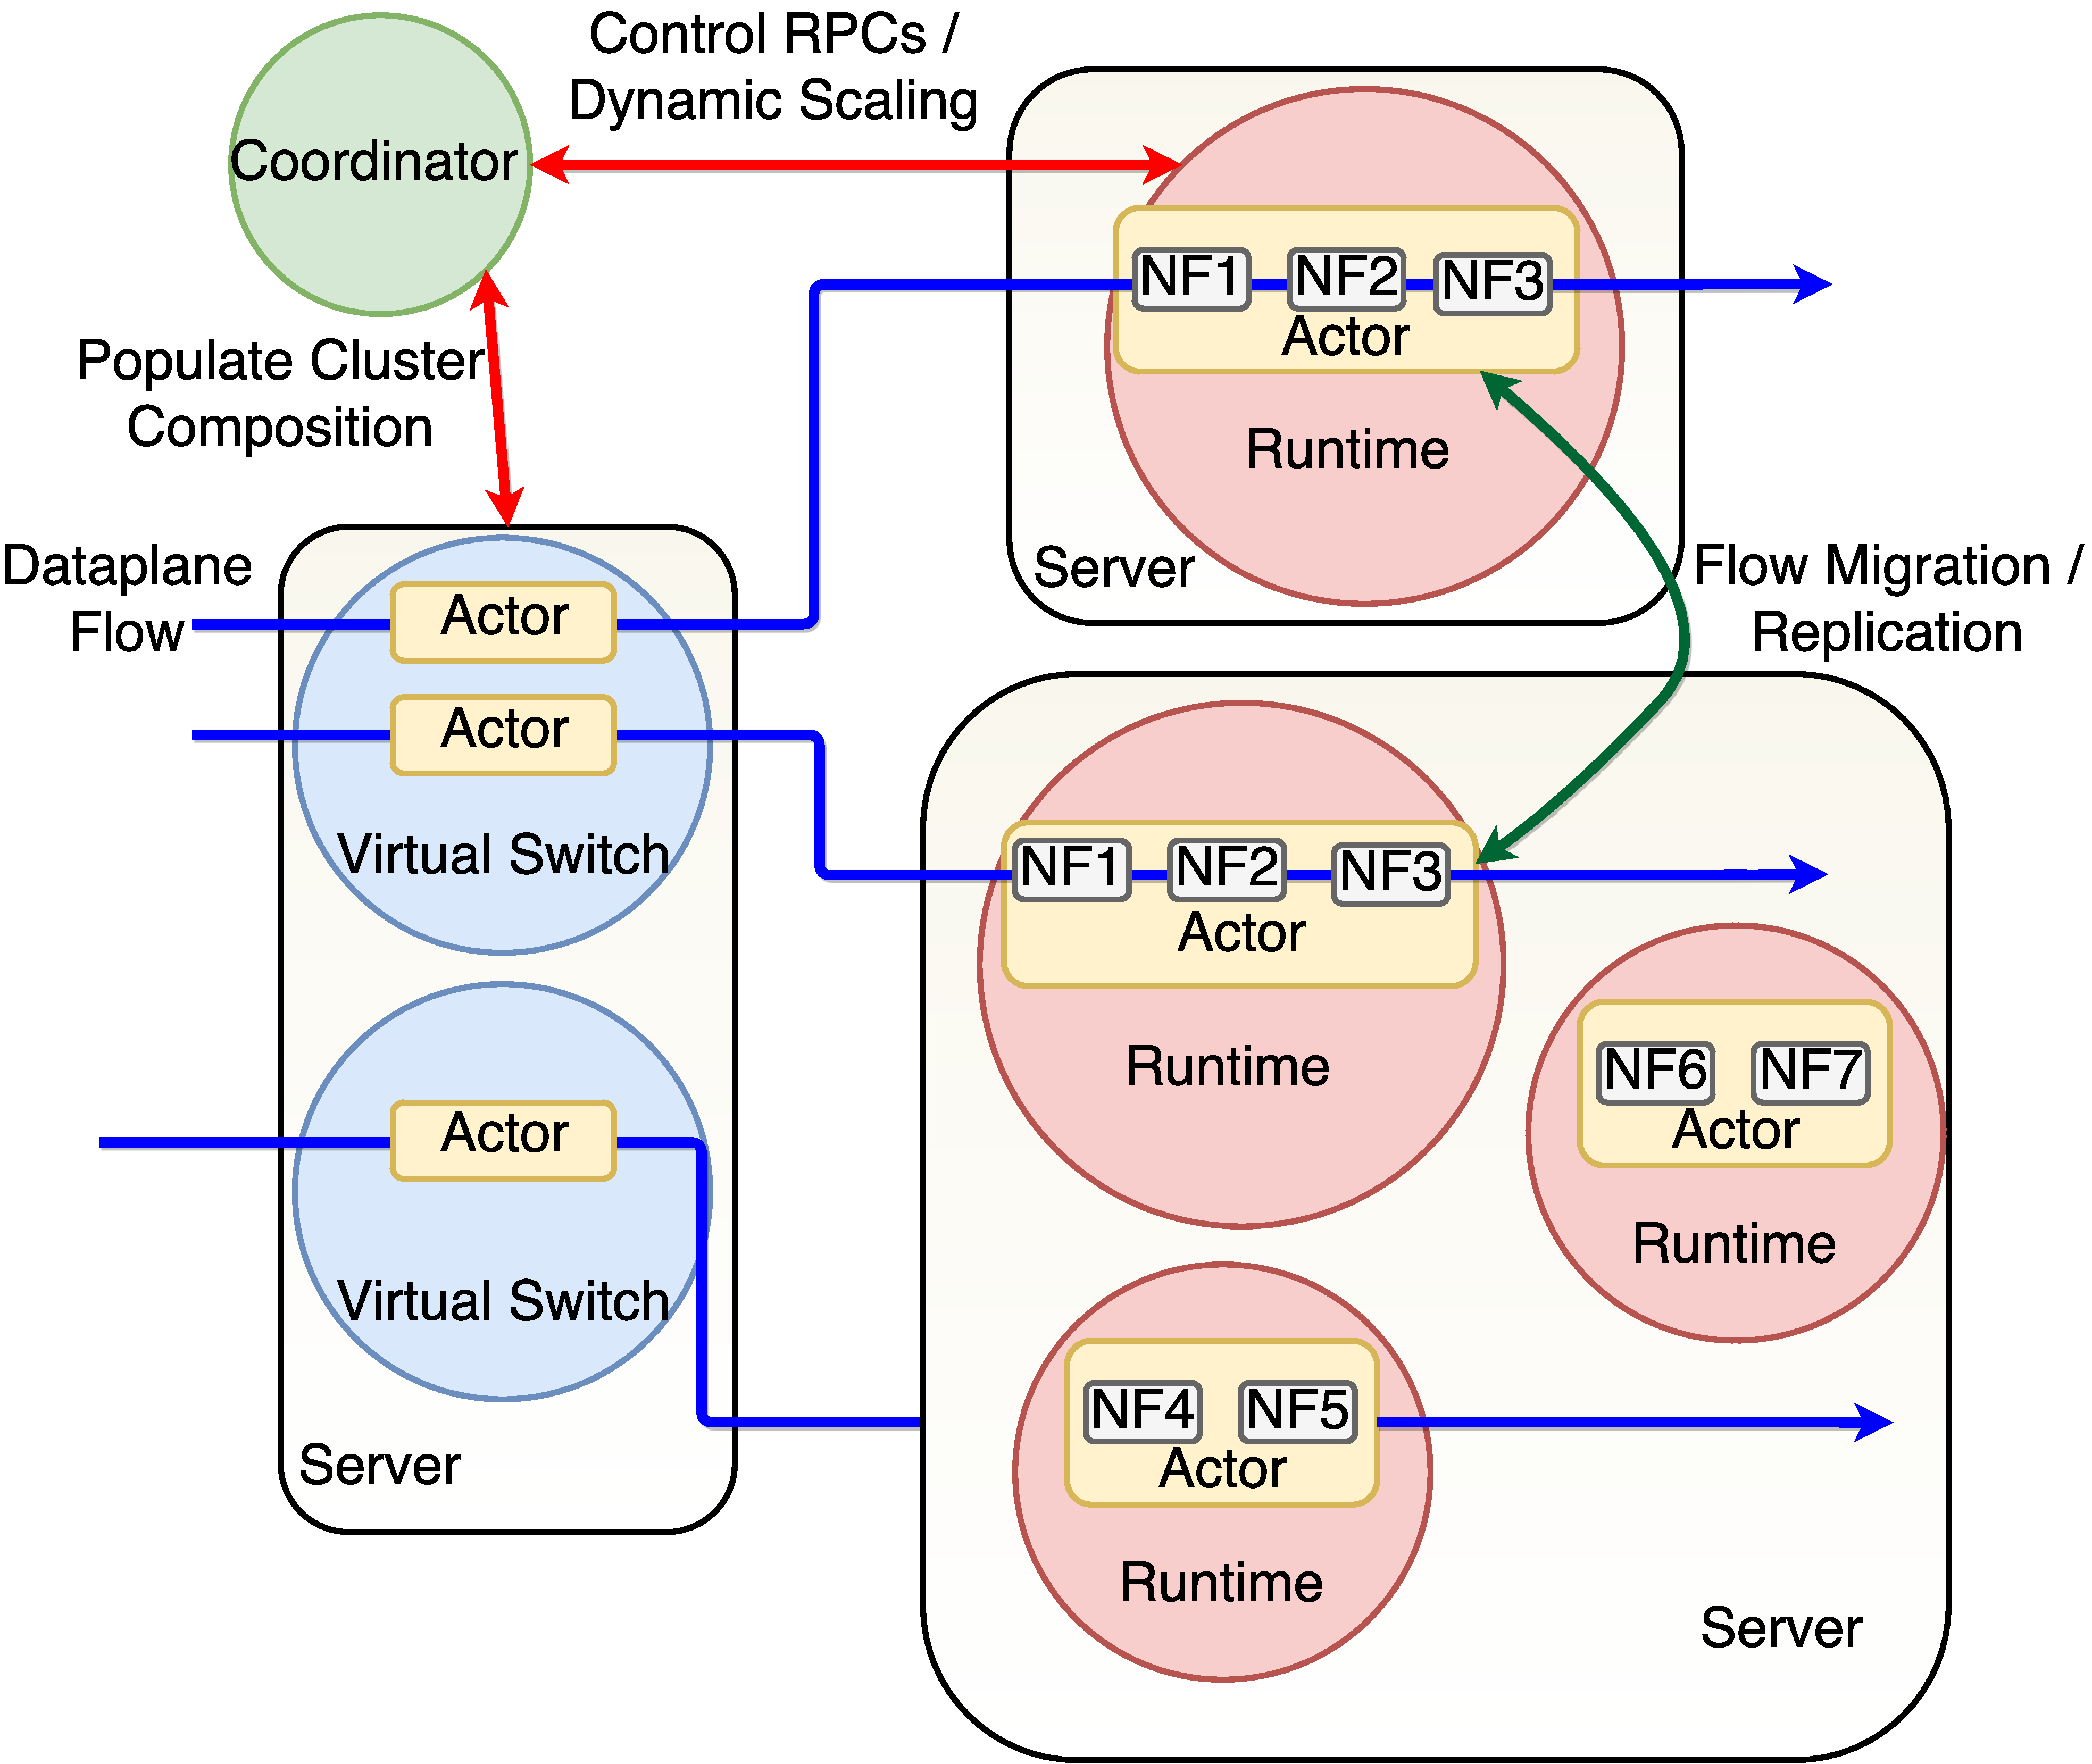
\includegraphics[width=\columnwidth]{chap-nfvactor/figure/new-nfactor-cluster.pdf}
  \caption{An overview of the basic components of \nfactor. Three clusters are shown in this figure: a cluster for provisioning service chain `NF1$\rightarrow$NF2$\rightarrow$NF3', a cluster for service chain `NF4$\rightarrow$NF5' and a cluster for service chain `NF6$\rightarrow$NF7'}
  \label{fig:runtime}
\end{figure}

\subsection{Overview}
\label{sec:overview}

At the highest level, \nfactor~has a layered structure as shown in Fig.~\ref{fig:runtime}. There are three key elements in~\nfactor: (i) runtime systems (referred to as \textit{runtime} for short) that enable flow processing using actors; (ii) virtual switches for distributing flows to runtime systems and sending flows to final destinations; and (iii) a lightweight coordinator for basic system management.

A runtime (Sec.~\ref{sec:runtime}) is the execution environment of flow actors, running on a Docker container \cite{docker} for quick launching and rebooting, and is assigned a globally unique ID upon creation. A virtual switch is a special runtime (Sec.~\ref{sec:virtualswitch}) and serves as the gateway to runtimes.
%Inside a physical server, runtimes and virtual switches are connected with a virtual L2 switch (L2Forward module of BESS \cite{bess}). Different physical servers are inter-connected through a physical Ethernet switch. In~\nfactor,
Runtimes and virtual switches are partitioned into several virtual clusters. In a cluster, the runtimes are initialized with the same service chain (Sec.~\ref{sec:rtsc}) and the virtual switches dispatch flows to the runtimes within the same cluster. The partitioning of virtual clusters enables~\nfactor~to simultaneously provision multiple service chains.

Each virtual switch is configured with an entry IP address. The coordinator sets up proper switching rules %SDN flow rules
to direct dataplane flows to virtual switches, which further dispatch them to runtimes within the same cluster. A runtime creates a dedicated flow actor to process each flow and forward flow packet to its final destination.
%After processing, the outgoing flow packets are sent to another virtual switch in the cluster, which forwards the flow to its final destination.
%\footnote{When our flow replication mechanism is in place, a flow will be sent by replica runtime to the virtual switch, to be forwarded outside (Sec.~\ref{sec:resilience}).}
The coordinator also manages dynamic scaling and failure recovery of~\nfactor~by interacting with runtimes and virtual switches through a series of control RPCs (Sec.~\ref{sec:coordinator}).

Dataplane flows can be migrated and replicated from one runtime to another runtime within the same cluster in a distributed fashion without persistent involvement of the coordinator. To replicate a flow (Sec.~\ref{sec:replicating-runtime}), the corresponding flow actor first launches a replica actor running on another runtime. Then the flow actor constantly saves its private state to the replica actor. The coordinator monitors the flow actor by regularly checking the liveness of the flow actor's runtime. In case of the runtime failure, the replica actor substitutes the flow actor and resumes normal flow processing. To migrate a flow (Sec.~\ref{sec:migration}), the flow actor initializes a target flow actor on another runtime. Then the flow actor contacts the virtual switch to redirect the flow to the target actor, followed by transmitting its private state to the target target. When the migration finishes, the original flow actor destroys itself and the target flow actor continues to process the flow.

\subsection{Runtime}
\label{sec:runtime}

\nfactor~employs a carefully designed, uniform runtime system to run flow actors. Within a runtime, we adopt a {\em one-actor-one-flow} design principle: a dedicated flow actor is created to handle each flow received by the runtime. Packet processing by NFs and resilience operations are all implemented as reactive message handlers of the flow actor. The runtime timely schedules each flow actor to react to the various events, so that each flow actor can process flow packets and manage its own resilience in a largely decentralized fashion. Our one-actor-one-flow principle improves the parallelism of resilience operations while the overhead for creating and managing per-flow actors is significantly reduced (Sec.~\ref{sec:micro-benchmark}) due to our efficient runtime design. This principle serves as the basis for high-performance resilience support.

%To further demonstrate how a runtime works, we first show the internal structure of a runtime, followed by its overall work flow to process data-plane flows and remote actor messages. Finally, we discuss the service chain model adopted by each runtime.

\subsubsection{Internal Structure}

\begin{figure}
		\centering
		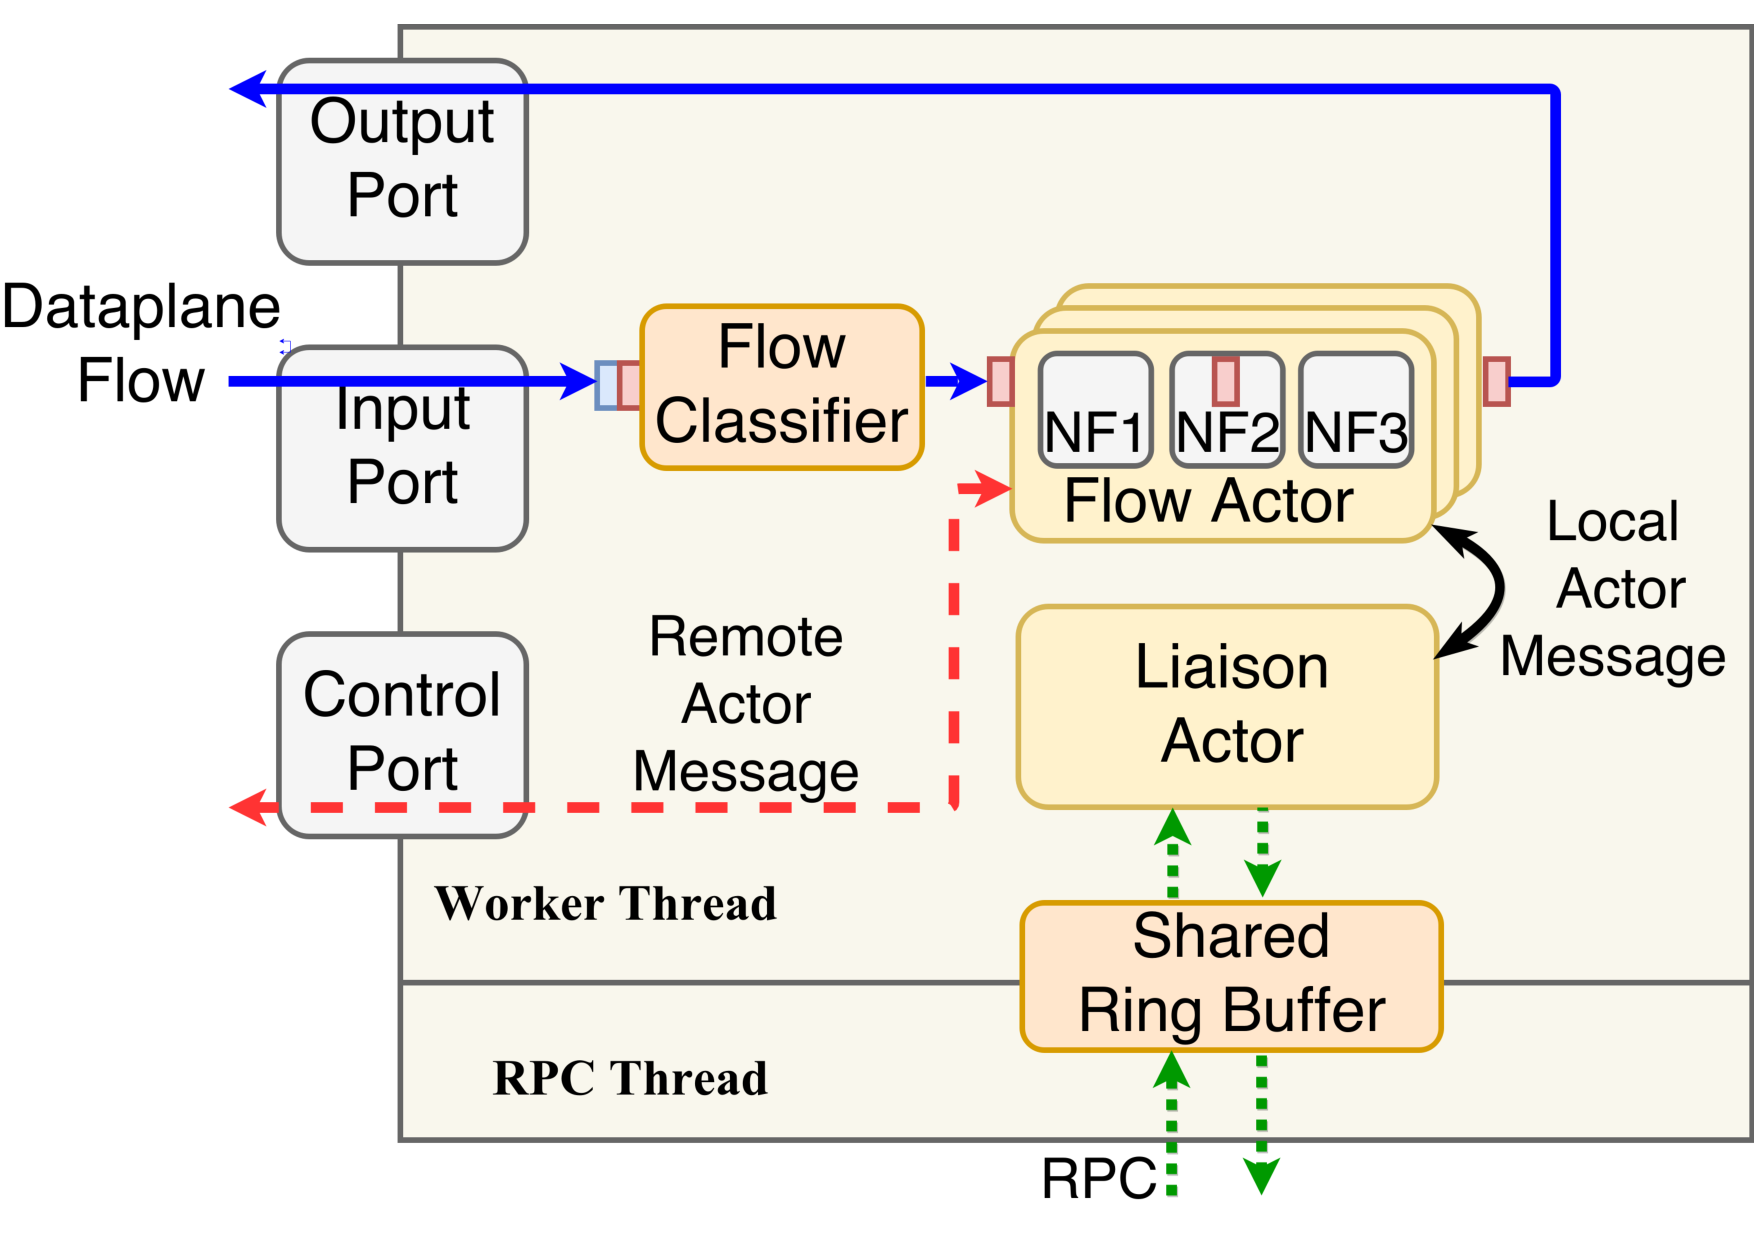
\includegraphics[width=\columnwidth]{chap-nfvactor/figure/new-nfactor-runtime-arch.pdf}
		\caption{The internal structure of a runtime.}
\label{fig:runtime-arch}
\end{figure}

Fig.~\ref{fig:runtime-arch} shows the internal structure of a runtime. Each runtime is configured with one worker thread and one RPC thread. The worker thread actively polls the three ports shown in Fig.~\ref{fig:runtime-arch} and is pinned to a dedicated CPU core to minimize the performance impact caused by thread scheduling. The RPC thread responds to RPC requests sent from the coordinator, for basic system management operations (Sec.~\ref{sec:coordinator}). The three ports are high-speed virtual NICs (ZeroCopyVPort in BESS \cite{bess}) and they are connected to a virtual L2 switch (L2Forward module of BESS) inside a physical server. The worker thread can bypass the kernel and directly fetch network packets from these ports.

\subsubsection{Work Flow}

The runtime has three basic work flows:

\noindent \textbf{Process Dataplane Flows:} The worker thread constantly polls dataplane flow packets from the input port. For each packet, the worker thread uses the 5-tuple of the packet (\ie, source IP address, destination IP address, transport-layer protocol, source port and destination port) to retrieve the corresponding flow actor and sends the packet to the flow actor for processing. Running in its own logical thread, the flow actor processes the packet along the configured service chain and then sends the processed packet out from the output port.

\noindent \textbf{Process Remote Actor Messages:} During distributed flow migration and replication, {\em remote actor messages} are exchanged among actors running on different runtimes. The runtime is equipped with a reliable message passing channel (Sec.~\ref{sec:nfvactor-implementation}) to reliably send and receive remote actor messages over the control port. The received remote actor messages are handed over to the destination actors for processing. The sent remote actor messages are reliably delivered to their receivers.

\noindent \textbf{Process Control RPCs:} The RPC thread forwards received RPC requests to a {\em liaison actor} in the worker thread through the shared ring buffer. The liaison actor coordinates with flow actors via {\em local actor messages}, to handle RPC requests sent from the coordinator.

%\textbf{Customized Actor Library:} To effectively run all these tasks while scheduling actors to react to events, we design a customized actor library (Sec.~\ref{sec:implementation}) for the runtime, equipped with a module graph scheduler and an user-space message passing channel. In Sec.~\ref{sec:micro-benchmark}, we show that our runtime significantly out-performs existing actor runtimes when scheduling actors to process network packets.

\subsubsection{Service Chain}
\label{sec:rtsc}

Each runtime is configured with a sequential service chain (\eg, firewall$\rightarrow$NAT$\rightarrow$load-balancer) and initializes all the NFs along the service chain upon booting. When the flow actor processes packets, it calls the $process\_pkt(input\_pkt, fs, ss)$ API (Sec.~\ref{sec:nfvactor-nf-api}) of each NF according to the service chain structure to implement the service chain processing logic.

%Due to the flexibility of the actor model, we believe that advanced service graph models \cite{OpenBox} can be easily embedded into~\nfactor~as well.

\subsection{Virtual Switch}
\label{sec:virtualswitch}

A virtual switch is a special runtime where the actors do not run service chains but only a flow forwarding function. An actor in a virtual switch is referred to as a {\em virtual switch actor}. The virtual switch serves as a load-balancing gateway when forwarding flows and a lightweight flow redirector when executing resilience operations.

For flow forwarding, a virtual switch learns runtimes that it can dispatch flows to through RPC requests sent from the coordinator. When a new flow arrives, a virtual switch actor selects a runtime with the smallest workload as the destination and saves its ID. For each flow packet, the virtual switch actor replaces the destination MAC address with the MAC address of the input port of the destination runtime and forwards the packet. %one of the runtimes to forward its flow according to the workload %in a round-robin fashion. A simple round-robin approach is adopted because it runs fast and~\nfactor~is able to effectively resolve hot-spots by flow migration. For subsequent flow packets, the virtual switch actor modifies their MAC address and forwards them to the selected runtime.

During flow migration and replication, each virtual switch actor can independently update the flow route by simply modifying the ID of the destination runtime. Compared with installing flow rules on an SDN switch \cite{rajagopalan2013split, gember2015opennf}, the route update process is lightweight and improves flow migration performance for~\nfactor.

\subsection{Coordinator}
\label{sec:coordinator}

\begin{table}[!h]
\centering
\caption{Control RPCs Exposed at Each Runtime}
\label{table:rpc}
\resizebox{\columnwidth}{!}{
\begin{tabular}{l|l}
\textbf{Control RPC}                                                                                   & \textbf{Functionality}                                                                                                                                              \\ \hline
poll\_workload()                                                                                   & \begin{tabular}[c]{@{}l@{}}Poll the load information \\ from a runtime.\end{tabular}                                                                 \\ \hline
notify\_cluster\_cfg(cfg)                                                                         & \begin{tabular}[c]{@{}l@{}}Notify a runtime/virtual switch  \\the current cluster composition.\end{tabular}                                                             \\ \hline
\begin{tabular}[c]{@{}l@{}}set\_migration\_target(runtime\_id, \\ migration\_number)\end{tabular} & \begin{tabular}[c]{@{}l@{}}Initiate flow migration. It tells \\ the runtime to migrate \\ migration\_num of flows to the \\ runtime with runtime\_id.\end{tabular} \\ \hline
set\_replicas(runtime\_id\_list)                                                                       & \begin{tabular}[c]{@{}l@{}}Set the runtimes with IDs  \\in runtime\_id\_list as the replica.\end{tabular}                                                                \\ \hline
recover(runtime\_id)                                                                          & \begin{tabular}[c]{@{}l@{}}Recover all the flows replicated \\ from runtime with runtime\_id.\end{tabular}                                                 \\ \hline
\end{tabular}
}
\end{table}


The coordinator in \nfactor~is responsible for basic cluster management routines, \eg, monitoring system workload, updating cluster composition,  dynamically scaling runtimes for deployed clusters, and recovering failed runtime in a cluster. As compared to centralized controllers in the existing NFV systems \cite{gember2015opennf, rajagopalan2013split}, the coordinator only uses light-weight RPC calls to initiate the flow migration and replication process.

The coordinator communicates with runtimes via a number of control RPCs summarized in Tbl.~\ref{table:rpc}. It uses $poll\_workload()$ to acquire the current workload on a runtime. It updates cluster composition (including MAC addresses of input/output/control ports, workload status and IDs of all runtimes and virtual switches in the cluster) to all the runtimes and virtual switches in a cluster using $notify\_cluster\_cfg(cfg)$.

To deploy a cluster, the system operator first specifies the composition of a service chain to the coordinator. The coordinator then creates a new cluster with one runtime and one virtual switch, configures the runtime with the specified service chain and installs proper switching rules to forward matching input flows to the virtual switch. The cluster is then dynamically scaled and recovered under the control of the coordinator.

The last three RPCs shown in Tbl.~\ref{table:rpc} are used to initiate flow migration and replication. After issuing these three calls, migration and replication are automatically executed among runtimes without further involving the coordinator.

%\subsection{Dynamic Scaling}
%\label{sec:scaling}

\textbf{Dynamic Scaling.} The coordinator performs dynamic scaling of the runtimes and virtual switches by exploiting the distributed flow migration mechanism. It fully exploits distributed flow migration mechanism to resolve hot spot and shut down mostly idle runtimes.

The coordinator periodically polls the workload statistics from all the runtimes, containing the number of dropped packets on the input port, the current packet processing throughput and the number of active flows. In the current~\nfactor~prototype, the runtime is identified as overloaded if the number of dropped packets exceeds a fixed threshold (100 as in our experiments). This is an effective overload indicator for~\nfactor: an overloaded runtime can not timely poll all the packets from its input port, therefore increasing the number of dropped packets significantly, while the CPU usage is rendered ineffective as the worker thread is a busy-polling thread and uses 100\% of the CPU all the time.

If there is an overloaded runtime in a cluster, the coordinator launches a new runtime in the same cluster and keeps migrating a configurable number of flows from overloaded runtime (500 as in our experiments) to the new runtime, until half of the workload on the overloaded runtime is migrated away. %all the hotspots are resolved. % If the new runtime becomes overloaded, more runtimes are added.
%We add new runtimes instead of moving flows across existing runtimes, since the load on existing runtimes is largely balanced, due to the load-balancing functionality of virtual switches.
If runtimes in a cluster become largely idle, the coordinator carries out scale-in: it selects a runtime with the smallest throughput, migrates all its flows to the other runtimes, and shuts the runtime down when all the flows have been successfully moved out.

%The coordinator periodically polls the load statistics from all the runtimes, containing the number of dropped packets on the input port, the current packet processing throughput and the number of active flows. Since the worker thread of the runtime is a busy-polling thread and uses 100\% of CPU all the time, CPU usage is not a good indicator to tell whether a runtime has been overloaded. In the current~\nfactor~prototype, the coordinator uses the total number of dropped packets on the input port of a runtime to determine overload, which is a very effective indicator in~\nfactor: an overloaded runtime can not timely poll all the packets from its input port, therefore increasing the number of dropped packets significantly. When the number of dropped packets per second exceeds 100, the runtime is identified as overloaded. If there is at least one overloaded runtime in a cluster, the coordinator launches a new runtime, configures it to run the same service chain, and keeps migrating a configurable number of flows from overloaded runtimes (500 as in our experiments) to the new runtime, until all the hotspots are resolved. If the new runtime becomes overloaded, more new runtimes are added. We add new runtimes instead of moving flows across existing runtimes, since the load on existing runtimes is largely balanced, due to the load-balancing functionality of virtual switches.
